%%%%%%%%%%%%%%%%%%%%%%%%%%%%%%%%%%%%%%%%%%%%%%%%%%%%%%%%%%%%%%%%%%%%%%%%% 
% $Id$
% %%%%%%%%%%%%%%%%%%%%%%%%%%%%%%%%%%%%%%%%%%%%%%%%%%%%%%%%%%%%%%%%%%%%%%%%%
%
% Set de slides estudiando diferencias entre uso de Green3D o Green2D
% para problema cilindro infinito usando una seccion (rodaja 3D) del
% cilindro
%
% %%%%%%%%%%%%%%%%%%%%%%%%%%%%%%%%%%%%%%%%%%%%%%%%%%%%%%%%%%%%%%%%%%%%%%%%%

% %%%%%%%%%%%%%%%%%%%%%%%%%%%%%%%%%%%%%%%%%%%%%%%%%%%%%%%%%%%%%%%%%%%%%%%%%
\subsection{FEM Formulation}
% %%%%%%%%%%%%%%%%%%%%%%%%%%%%%%%%%%%%%%%%%%%%%%%%%%%%%%%%%%%%%%%%%%%%%%%%%

\begin{frame}[allowframebreaks]{Formulation}
  \begin{columns}
    \column{0.4\textwidth} \centering
    {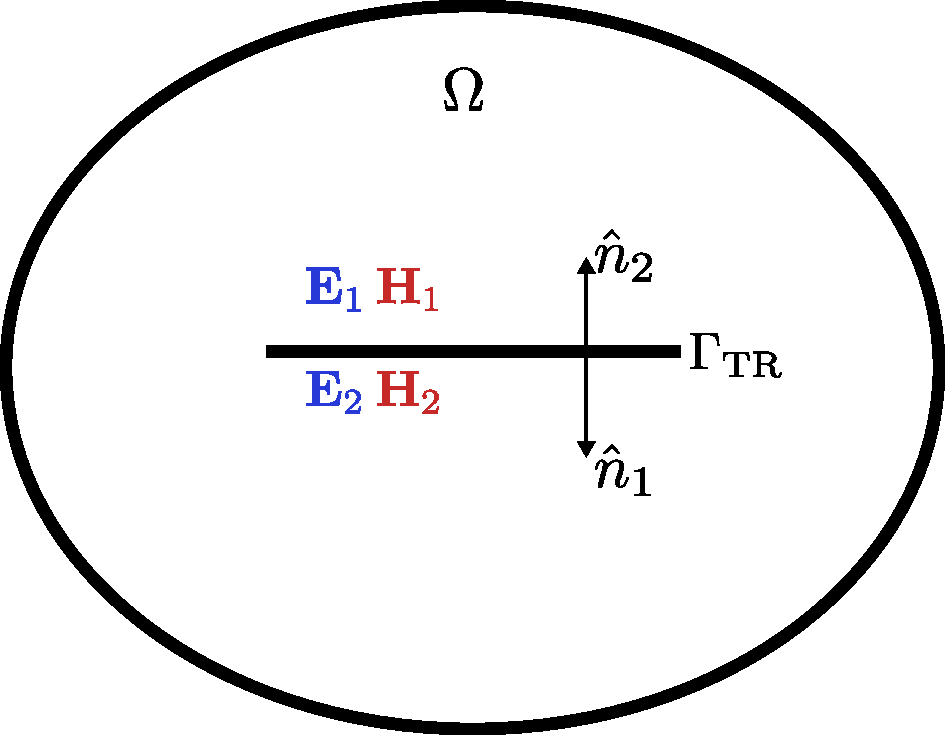
\includegraphics[angle=0,width=\textwidth]{scenario.pdf}}
    \column{0.6\textwidth}
    {
      \begin{align*}
        \hat{n}_1\times(\mu_r^{-1}&\nabla\times\vec{E}_1) - \frac{jk_0}{\eta}y_{11}\hat{n}_1\times(\hat{n}_1\times\vec{E}_1) - \\
        - &\frac{jk_0}{\eta}y_{12}\hat{n}_2\times(\hat{n}_2\times\vec{E}_2) = 0,
      \end{align*}
      \begin{align*}
        \hat{n}_2\times(\mu_r^{-1}&\nabla\times\vec{E}_2) - \frac{jk_0}{\eta}y_{21}\hat{n}_1\times(\hat{n}_1\times\vec{E}_1) - \\
        - &\frac{jk_0}{\eta}y_{22}\hat{n}_2\times(\hat{n}_2\times\vec{E}_2) = 0,
      \end{align*}

      \alert{Note that $y_{\rm xx}$ are relative to the vacuum admittance.}
    }
  \end{columns}

  \framebreak % %%%%%%%%%%%%%%%%%%%%%%%%%%%%%%%%%%%%%%

  Find $\vec{E} \in \vec{H}_0(\text{curl},\Omega)$ such that
  \begin{align*}
    &\Big(\nabla\times\vec{w},\mu_r^{-1}\nabla\times\vec{E} \Big)_\Omega - k_0^2\Big(\vec{w},\varepsilon_r\vec{E} \Big)_\Omega + 
    jk_0\Big\langle\hat{n}\times\vec{w},\hat{n}\times\vec{w}\Big\rangle_{\Gamma_{\text{C}}} = \\
    &\;\Big(\vec{w},\vec{F}\Big)_\Omega - 
    \Big\langle\hat{n}\times(\vec{w}\times\hat{n}),\vec{\Psi}_{\text{N}}\Big\rangle_{\Gamma_{\text{N}}} -
    \Big\langle\hat{n}\times(\vec{w}\times\hat{n}),\vec{\Psi}_{\text{C}}\Big\rangle_{\Gamma_{\text{C}}}
    \quad \forall \,\vec{w} \in \vec{H}_0(\text{curl},\Omega).
  \end{align*}
  
  with
  \begin{align}
    \Big(\vec{w},\vec{v}\Big)_\Omega &= \int_\Omega \vec{w}^* \cdot \vec{v} d\Omega, \nonumber\\
    \Big\langle \vec{w},\vec{v}\Big\rangle_{\Gamma} &= \int_\Gamma \vec{w}^* \cdot \vec{v} d\Gamma.\nonumber
  \end{align}
  
  \framebreak % %%%%%%%%%%%%%%%%%%%%%%%%%%%%%%%%%%%%%%
  For \emph{upper} elements on $\Gamma_{\rm TR}$ (side 1), we have
  \small
  \begin{align*}
    &{\rm LHS_1} \\
    &\; + j\frac{k_0}{\eta}\Big\langle\hat{n}\times(\vec{w}_1\times\hat{n}),y_{11}\hat{n}\times(\vec{w}_1\times\hat{n})\Big\rangle_{\Gamma_{\text{TR}}} + j\frac{k_0}{\eta}\Big\langle\hat{n}\times(\vec{w}_1\times\hat{n}),y_{12}\hat{n}\times(\vec{w}_2\times\hat{n})\Big\rangle_{\Gamma_{\text{TR}}} = \\
    &\;\;{\rm RHS_1},
  \end{align*}
  \normalfont
  whereas for \emph{lower} elements (side 2), we get
  \small
  \begin{align*}
    &{\rm LHS_2} \\
    &\; + j\frac{k_0}{\eta}\Big\langle\hat{n}\times(\vec{w}_2\times\hat{n}),y_{21}\hat{n}\times(\vec{w}_1\times\hat{n})\Big\rangle_{\Gamma_{\text{TR}}} + j\frac{k_0}{\eta}\Big\langle\hat{n}\times(\vec{w}_2\times\hat{n}),y_{22}\hat{n}\times(\vec{w}_2\times\hat{n})\Big\rangle_{\Gamma_{\text{TR}}} = \\
    &\;\;{\rm RHS_2},
  \end{align*}
  \normalfont
\end{frame}

\begin{frame}{FEM implementation}
  \begin{itemize}
    \item The DOFs will be doubled for the faces and the interior edges.
    \item The exterior edges of $\Gamma_{\rm TR}$ are not doubled.
    \begin{itemize}
      \item Identified by code: the edges associated to two faces are interior. 
      \item If the boundaries of the sheet belong to PBC, the edges of $\Gamma_{\rm TR}$ are also doubled.
    \end{itemize}
  \end{itemize}
\end{frame}

% %%%%%%%%%%%%%%%%%%%%%%%%%%%%%%%%%%%%%%%%%%%%%%%%%%%%%%%%%%%%%%%%%%%%%%%%%
\subsection{Testing}
% %%%%%%%%%%%%%%%%%%%%%%%%%%%%%%%%%%%%%%%%%%%%%%%%%%%%%%%%%%%%%%%%%%%%%%%%%

\begin{frame}{Problem to be solved}
  \begin{columns}
    \column{0.48\textwidth} \centering
    {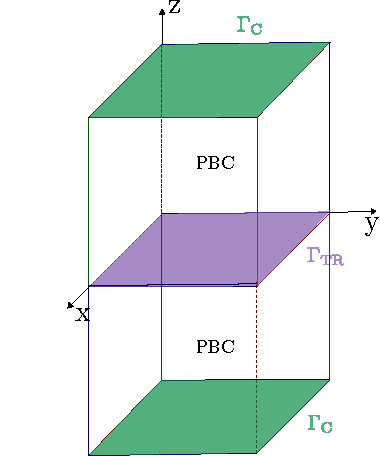
\includegraphics[angle=0,width=\textwidth]{tr_problem.pdf}}
    \column{0.48\textwidth}
    {
      Simulation of an infinite medium with transmission/reflection sheet that divides the space into two halves.
      \begin{itemize}
        \item $\Gamma_\text{TR}$: Transmission/reflection sheet defined with 
        \begin{equation*}
          \vec{Y} = \begin{bmatrix}
            y_{11} & y_{12} \\
            y_{21} & y_{22}
          \end{bmatrix}.
        \end{equation*}
        \item $\Gamma_\text{C}$: ABC with excitation with polarization $E_y$
        \item The vertical faces are set to PBC
      \end{itemize} 
    }
  \end{columns}
\end{frame}

\begin{frame}{Testbench}
  \begin{itemize} 
    \item $\vec{Y} = \begin{bmatrix}
      0 & 0 \\
      0 & 0
    \end{bmatrix}$: sanity check, we should get same result as the two halves with a PMC.
    \item $\vec{Y} = \mathbb{I}$: sanity check, we should get same result as the two halves with an ABC.
    \item Change lower $\Gamma_\text{C}$ by PEC and solve analytic problem with four media: final test.
    \begin{itemize}
      \item Obtain parameters for $\vec{Y}$ of the equivalent problem.
      \item Get same solutions for the electric field.
      \item Transparent? Puede ser que aproximar con $1e6$. Quizás con ABCD.
    \end{itemize}
  \end{itemize}
\end{frame}

% %%%%%%%%%%%%%%%%%%%%%%%%%%%%%%%%%%%%%%%%%%%%%%%%%%%%%%%%%%%%%%%%%%%%%%%%%
\subsection{HOFEM Implementation}
% %%%%%%%%%%%%%%%%%%%%%%%%%%%%%%%%%%%%%%%%%%%%%%%%%%%%%%%%%%%%%%%%%%%%%%%%%

\begin{frame}{HOFEM implementation}
  \begin{itemize}
    \item New boundary condition: \texttt{TRBC}.
    \begin{itemize}
      \item We define a normal, $\hat{n}_{\rm TRBC}$ to detect lower and upper side. Upper side is the closer to $\hat{n}_{\rm TRBC}$.
      \item Definition of $y_{11}$, $y_{12}$, $y_{21}$, and $y_{22}$ as relative values with respect to vacuum admittance.
    \end{itemize}
    \item Two options for implementation 
    \begin{itemize}
      \item Integers defined in \texttt{tetrahedra\_element}.
      \item Allocatable array of $1\times N_{\rm elem, TR}$ where the two positions (stored in boundary conditions module, 
      accessible from \texttt{mesh\_reordering\_module} and \texttt{elementary\_terms\_3D}):
      \begin{enumerate}
        \item $10\times$ Neighbor element identifier (to couple $\vec{w}_2$ and $\vec{w}_1$).
        \item Integer 1,2 (side) (to extract the values of $y_{11}$,$y_{12}$,$y_{21}$, and $y_{22}$).
        % \item Integer 10\texttt{bc\_id}+[1,2] (side) (to extract the values of $y_{11}$,$y_{12}$,$y_{21}$, and $y_{22}$).
      \end{enumerate}
      % the neighbor for elements belonging to $\hat{n}_{\rm TRBC}$ and an integer 10\texttt{bc\_id}+[1,2] (side), located in \texttt{mesh\_object\_module}, accessible from \texttt{mesh\_reordering\_module} and \texttt{elementary\_terms\_3D}.
    \end{itemize}
    \item Significant methods involved:
    \begin{itemize}
      \item Postprocessing over \texttt{reordering\_DOF\_algorithm\_3D}. 
      \item \texttt{calc\_boundary\_3D\_nxNi\_nxNi\_term\_of\_this\_element}.
      \item Construction of the MUMPS-related matrix: different number of
      non-zeros per element, assembly of coupled elements (now single-element
      assembly).
    \end{itemize}   
  \end{itemize}
\end{frame}
%%%%%%%%%%%%%%%%%%%%%%%%%%%%%%%%%%%%%%%%%%%%%%%%%%%%%%%%%%%%%%%%
